\chapter{Results}
\com{
\todo[inline]{
Sometimes this is split into two chapters.\\

Keep in mind: How you are going to evaluate what you have done? What are your metrics?\\
Analysis of your data and proposed solution\\
Does this meet the goals which you had when you started?
}
}
\label{ch:results}


\noindent
The results as obtained by the evaluation techniques of the localisation and mapping feature are shown in this chapter.
The different configurations for the localisation module are defined and analysed using both the gravel training and grass validation runs.
Some considerations are proposed in relation to the improvements provided.
The mapping module performance is evaluated by showing the results obtained using both the virtual boundary definition and the map update features.
The final discussion wraps up the key findings identified by both the runs.


\section{Localisation Analysis}
\label{sec:locRes}
\noindent
The localisation module is evaluated by comparing different sensors' configurations.
Each configuration provides different performance for the \gls{EKF} filter.
The selections proposed have been thought as improvements of the original \gls{HRP}, trying to exploit the measurements of the newly added sensors.
The initial model is given by the raw \gls{GPS} measurements and it is provided as reference.
The first configured model is defined using the original configuration of sensors.
The addition of the \glspl{IMU} is then accounted for in the next model, and consequentially, also the addition of the results from the \gls{VO} is considered for the complete configuration.
The following models are configured so that the control input is not considered, as it could happen if the localisation module was provided as an external module with no access to the control information.
The models analysed by the experiments are summarised below in Table \ref{tab:eval-models}, along with the related brief description. 
\begin{table}[!ht]
	\small
	\begin{center}
		
		\begin{tabular}{|c||c|c|c|c|c|c|}
			\hline
			\multirow{2}{*}{\textbf{Model}} & \multicolumn{5}{c|}{\textbf{Sensors}} & \multirow{2}{*}{\textbf{Description}}\\
			& \multicolumn{1}{c|}{Control} & \multicolumn{1}{c|}{\gls{WO}} & \multicolumn{1}{c|}{\gls{GPS}} & \multicolumn{1}{c|}{\glspl{IMU}} & \multicolumn{1}{c|}{\gls{VO}} & \\
			\hline
			\hline
			\centering{GPS} &  & & $[x, y, \theta]$ &   &   & Raw measurements. \\
			\hline
			\centering{1} & $[v, \omega]$ & $[v, \omega]$ & $[x, y]$ &   &   & Original sensors ...  \\
			\hline
			\centering{2} & $[v, \omega]$ & $[v, \omega]$ & $[x, y]$ & $[\omega]$ &  & ~~ ... plus IMUs . ~~\\
			\hline
			\centering{3} & $[v, \omega]$ & $[v, \omega]$ & $[x, y]$ & $[\omega]$ & $[v, \omega]$  & Complete . ~~~~~ \\
			\hline
			\centering{4} & & $[v, \omega]$ & $[x, y]$ &  &   & No Control ... ~~~ \\
			\hline
			\centering{5} &  & $[v, \omega]$ & $[x, y]$ & $[\omega]$ &  &  IMUs over Control ... \\
			\hline
			\centering{6} &  & $[v, \omega]$ & $[x, y]$ & $[\omega]$  & $[v, \omega]$  & ~~ ... plus VO . \\
			\hline
			\centering{7} &  & $[v, \omega]$ & $[x, y, \theta]$ & $[\omega]$  &  & Proposed approach . \\
			\hline
			\hline
		\end{tabular}
		\caption{Experiments configuration.\label{tab:eval-models}}
	\end{center}
\end{table}

\subsection{Gravel Test Experiment }
\noindent This test was run on an even ground with gravel.
It has been the first extensive and comprehensive experiment run with all the measurements available.
The following localisation performance have been obtained by executing the different configurations of sensors and retrieving their localisation evaluations.
The estimates of all the modules are shown as obtained at each step by them in Figure \ref{fig:gravel-model}.
\begin{figure}[!ht]
			\begin{center}
				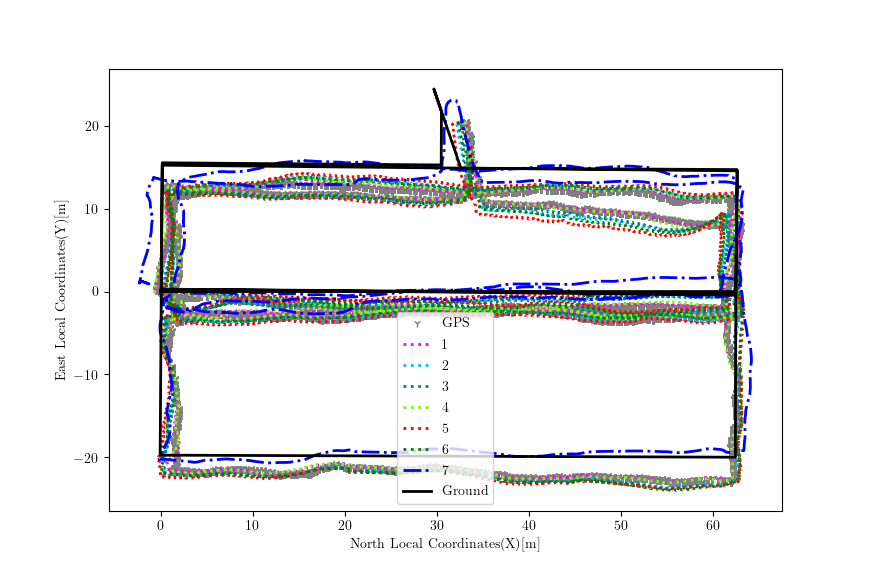
\includegraphics[clip , width=1 \textwidth]{Images/5-Results/GravelLoc.png} % , trim=2cm 1cm 2cm 0.8cm
			\end{center}
			\caption{Comparison of the localisation estimates of six different models on gravel\com{, plus the raw \gls{GPS} position fixes}.\label{fig:gravel-model}}
\end{figure}
%\\~\\

These results of each model, as obtained by averaging the metrics computed at each step, are shown in Table \ref{tab:grav-rmse}.
	\begin{table}[!ht]
		\small
		\begin{center}
			\begin{tabular}{|c|||S[table-format=-1.2]|S[table-format=-1.2]|S[table-format=-1.2]||S[table-format=-1.1(1)]|}
				\hline
				\multirow{3}{*}{\textbf{Model}} & \multicolumn{4}{c|}{\textbf{Evaluation Criteria}} \\
				& \multicolumn{3}{c||}{\textbf{RMSE}} & \multicolumn{1}{c|}{\textbf{Sampling period}}\\
			    & \multicolumn{1}{c|}{$\mathbf{x}$[\SI{}{\meter}]} & \multicolumn{1}{c|}{$\mathbf{y}$[\SI{}{\meter}]} & \multicolumn{1}{c||}{$\boldsymbol \theta$[\SI{}{\radian}]} & \multicolumn{1}{c|}{$\Delta_t \pm \sigma_{\boldsymbol \Delta_t}$ [\SI{}{\milli \second}]} \\
				\hline
				\hline
				\centering{GPS} & 1.33 & 2.88 & 0.76 & 1014 \pm 67 \\
				\hline
				\centering{1} & 1.11 & 2.75  & 0.31 & 11.6 \pm 4.0 \\
				\hline
				\centering{2} & 0.98 & 2.79 & 0.38 & 12.1 \pm 4.1 \\
				\hline
				\centering{3} & 1.03 & 2.77 & 0.35 & 12.0 \pm 4.3 \\
				\hline
				\centering{4} & 1.05 & 2.73 & 0.34 & 11.7 \pm 4.0 \\
				\hline
				\centering{5} & 0.92 & 2.83 & 0.42 & 11.9 \pm 3.9 \\
				\hline
				\centering{6} & 1.00 & 2.77 & 0.36 & 12.0 \pm 4.0 \\
				\hline
				\centering{7} & 0.95 & 1.18 & 0.51 & 10.1 \pm 5.1 \\
				\hline
			\end{tabular}
			\caption{Gravel experiment results.\label{tab:grav-rmse}}
		\end{center}
	\end{table}

The final poses' offsets as obtained by the different models, along with their related estimated standard deviation, are shown in Table \ref{tab:final-gravel}.
	\begin{table}[!ht]
		\small
		\begin{center}
			\begin{tabular}{|c||S[table-format=-1.2(4)]|S[table-format=-1.2(1)]|S[table-format=-1.2(1)]|}
				\hline
				\multirow{2}{*}{\textbf{Model}} & \multicolumn{3}{c|}{\textbf{Final Offset $\pm$ Uncertainty}} \\
				& \multicolumn{1}{c|}{$\mathbf{x} \pm \sigma_\mathbf{x}$[\SI{}{\meter}]} & \multicolumn{1}{c|}{$\mathbf{y} \pm \sigma_\mathbf{y}$[\SI{}{\meter}]} & \multicolumn{1}{c|}{$\boldsymbol \theta  \pm \sigma_{\boldsymbol \theta}$[\SI{}{\radian}]} \\
				\hline
				\hline
				\centering{GPS} & 0.38 \pm 3.25 & 0.50 \pm 3.25 & 0.58 \pm 0.27 \\
				\hline
				\centering{1} & 0.36 \pm 0.58 & 0.60 \pm 1.39 & 0.57 \pm 0.04 \\
				\hline
				\centering{2} & 0.51 \pm 0.62 & 0.68 \pm 0.55 & 0.54 \pm 0.01 \\
				\hline
				\centering{3} & 0.41 \pm 0.47 & 0.72 \pm 0.55 & 0.57 \pm 0.54 \\
				\hline
				\centering{4} & 0.37 \pm 0.20 & 0.65  \pm 0.89 & 0.84 \pm 0.04 \\
				\hline
				\centering{5} & 0.58 \pm 0.37 & 0.72  \pm 0.33 & 0.42 \pm 0.01 \\
				\hline
				\centering{6} & 0.48 \pm 0.29 & 0.66 \pm 0.31 & 0.55 \pm 0.01 \\
				\hline
				\centering{7} & 1.32 \pm 0.41 & 0.38 \pm 0.39 & 0.26 \pm 0.01 \\
				\hline
			\end{tabular}
			\caption{Gravel experiment final results.\label{tab:final-gravel}}
		\end{center}
	\end{table}



\com{
\begin{figure}[!ht]
	\begin{center}
		\begin{subfigure}[b]{.495\textwidth}
			\begin{center}
				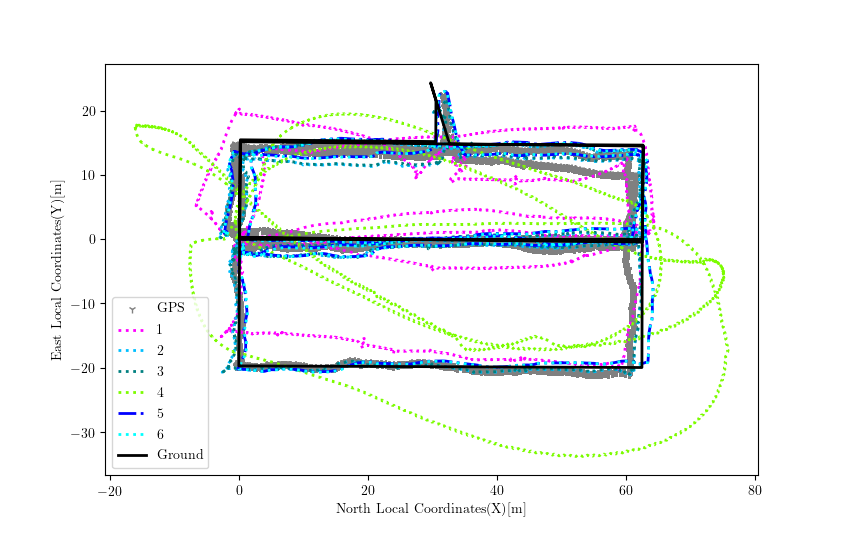
\includegraphics[width=1\textwidth]{Images/5-Results/Gravel-KF.png}
			\end{center}
			\caption{Different filters comparison}
			\label{fig:d435}
		\end{subfigure}
		\begin{subfigure}[b]{.495\textwidth}
			\begin{center}
				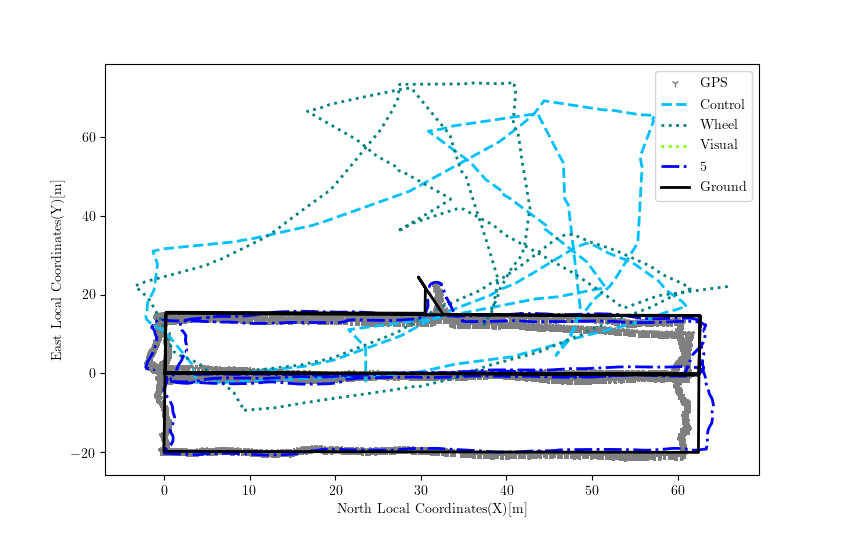
\includegraphics[width=1\textwidth]{Images/5-Results/Gravel-Loc.png}
			\end{center}
			\caption{Best filter performance}
			\label{fig:d435}
		\end{subfigure}%
		\caption{Localisation on gravel results.}
		\label{fig:camera_sensor}
	\end{center}
\end{figure}
}


\subsection{Grass Validation Experiment }
\noindent
This test was run on an even ground with long grass.
This experiment is run using the same techniques, defined in the Method chapter, adopted for the previous experiment.
This has been done to try to validate the calibration and localisation performance provided by the same models on different settings.

The following localisation performance have been obtained by executing the different configurations of sensors and retrieving their localisation evaluations, as before.
%\\~\\
The estimates of all the modules are shown as obtained at each step by them in Figure \ref{fig:grass-models}.
\begin{figure}[!ht]
			\begin{center}
				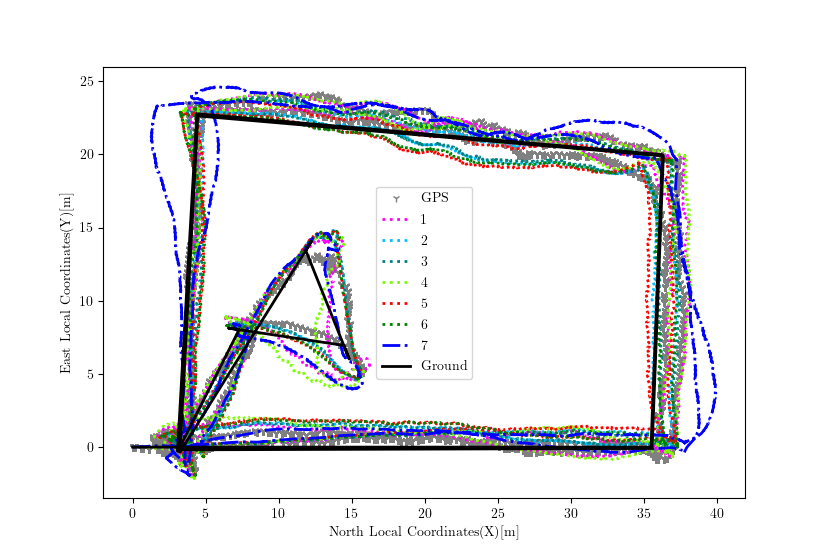
\includegraphics[clip, width=1 \textwidth]{Images/5-Results/GrassLoc.png} %, trim=2cm 1cm 2cm 0.8cm
			\end{center}
			\caption{Comparison of the localisation estimates of different models on grass.}
	\label{fig:grass-models}
\end{figure}

These results of each model, as obtained by averaging the metrics computed at each step, are shown in Table \ref{tab:grass-eval}.
	\begin{table}[!ht]
		\small
		\begin{center}
			\begin{tabular}{|c|||S[table-format=-1.2]|S[table-format=-1.2]|S[table-format=-1.2]||S[table-format=-1.2(1)]|}
				\hline
				\multirow{3}{*}{\textbf{Model}} & \multicolumn{4}{c|}{\textbf{Evaluation Criteria}} \\
				& \multicolumn{3}{c||}{\textbf{RMSE}} & \multicolumn{1}{c|}{\textbf{Sampling period}}\\
			    & \multicolumn{1}{c|}{$\mathbf{x}$[\SI{}{\meter}]} & \multicolumn{1}{c|}{$\mathbf{y}$[\SI{}{\meter}]} & \multicolumn{1}{c||}{$\boldsymbol \theta$[\SI{}{\radian}]} & \multicolumn{1}{c|}{$\Delta_t \pm \sigma_{\boldsymbol \Delta_t}$ [\SI{}{\milli \second}]} \\
				\hline
				\hline
				\centering{GPS} & 1.86 & 1.33 & 0.84 & 1020 \pm 74 \\
				\hline
				\centering{1} & 1.68 & 1.49  & 0.37  & 10.3 \pm 3.5 \\
				\hline
				\centering{2} & 1.58 & 1.44 & 0.26 & 10.8 \pm 3.8 \\
				\hline
				\centering{3} & 1.50 & 1.41 & 0.21 & 10.8 \pm 3.8 \\
				\hline
				\centering{4} & 1.84 & 1.60 & 0.40 & 10.3 \pm 3.5 \\
				\hline
				\centering{5} & 1.81 & 1.55 & 0.30 & 10.9 \pm 3.8 \\
				\hline
				\centering{6} & 1.66 & 1.49 & 0.25 & 10.9 \pm 3.8 \\
				\hline
				\centering{7} & 1.49 & 0.89 & 0.47 & 9.5 \pm 7.0 \\
				\hline
			\end{tabular}
			\caption{Grass experiment results.\label{tab:grass-eval}}
		\end{center}
	\end{table}
%\\~\\~\\~\\~\\

The final poses' offsets as obtained by the different models, along with their related estimated standard deviation, are shown in Table \ref{tab:grass-final}.
	\begin{table}[!ht]
		\small
		\begin{center}
			\begin{tabular}{|c||S[table-format=-1.2(4)]|S[table-format=-1.2(1)]|S[table-format=-1.2(1)]|}
				\hline
				\multirow{2}{*}{\textbf{Model}} & \multicolumn{3}{c|}{\textbf{Final Offset $\pm$ Uncertainty}} \\
				& \multicolumn{1}{c|}{$\mathbf{x} \pm \sigma_\mathbf{x}$[\SI{}{\meter}]} & \multicolumn{1}{c|}{$\mathbf{y} \pm \sigma_\mathbf{y}$[\SI{}{\meter}]} & \multicolumn{1}{c|}{$\boldsymbol \theta  \pm \sigma_{\boldsymbol \theta}$[\SI{}{\radian}]} \\
				\hline
				\hline
				\centering{GPS} & 1.47 \pm 2.50 & 0.14 \pm 2.50 & 0.62 \pm 0.20 \\
				\hline
				\centering{1} & 1.35 \pm 0.35 & 0.20 \pm 1.37 & 0.59 \pm 0.01 \\
				\hline
				\centering{2} & 1.44 \pm 0.19 & 0.23 \pm 0.81 & 0.58 \pm 0.01 \\
				\hline
				\centering{3} & 1.43 \pm 0.18 & 0.24 \pm 0.80 & 0.58 \pm 0.01\\
				\hline
				\centering{4} & 1.31 \pm 0.30 & 0.17 \pm 0.74 & 0.60 \pm 0.02 \\
				\hline
				\centering{5} & 1.36 \pm 0.15 & 0.21 \pm 0.46 & 0.59 \pm 0.01 \\
				\hline
				\centering{6} & 1.36 \pm 0.15 & 0.21 \pm 0.46 & 0.59 \pm 0.01 \\
				\hline
				\centering{7} & 1.34 \pm 0.06 & 0.14 \pm 0.06 & 0.60 \pm 0.02 \\
				\hline
			\end{tabular}
			\caption{Grass experiment final results.
			\label{tab:grass-final}}
		\end{center}
	\end{table}
	

\com{
\begin{figure}[!ht]
	\begin{center}
		\begin{subfigure}[b]{.495\textwidth}
			\begin{center}
				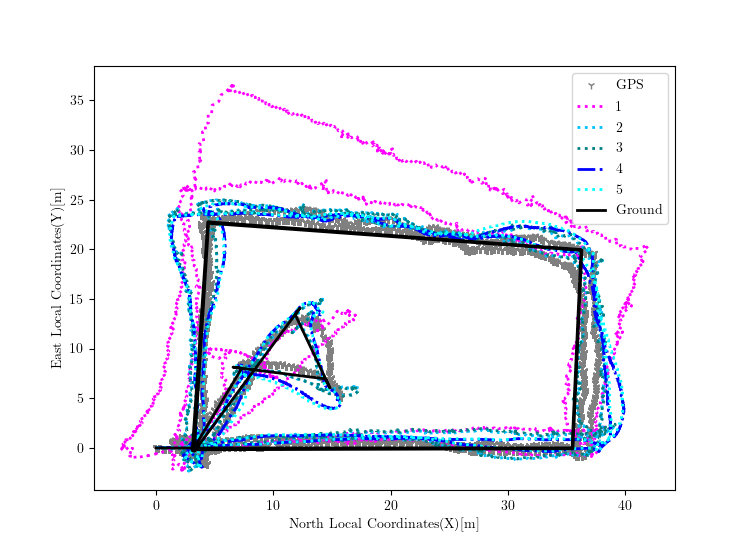
\includegraphics[width=1\textwidth]{Images/5-Results/Grass4-KF.png}
			\end{center}
			\caption{Different filter comparison}
			\label{fig:d435}
		\end{subfigure}
		\begin{subfigure}[b]{.495\textwidth}
			\begin{center}
				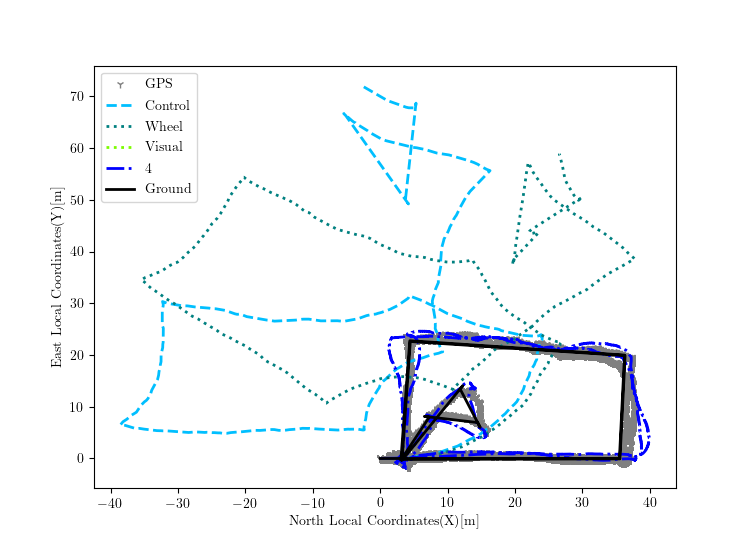
\includegraphics[width=1\textwidth]{Images/5-Results/Grass4-Loc.png}
			\end{center}
			\caption{Best filter performance}
			\label{fig:d435}
		\end{subfigure}%
		\caption{Localisation on grass results }
		\label{fig:camera_sensor}
	\end{center}
\end{figure}
}


\subsection{Discussion on Localisation}
\noindent
Using a sensor fusion approach, such as \gls{EKF}, it is possible to improve the localisation performance of an \gls{ALM}.
The results show how the localisation's configuration improves the estimate of the pose in real-time with respect to the \gls{GPS} receiver raw measurements.
The best positioning module is obtained by not considering control, adopting an orientation model for the \gls{GPS} and adding \glspl{IMU}, which are exploited to improve the angular velocity estimation and to model the process system noise in the prediction step of the \gls{EKF}. % with a configuration which enables for dynamic system noise generation.
The sensor fusion with an adaptive approach manages to provide the best performance using the available sensors.
It exploits the varying noise parameters determining them at each step, which are based on the measurements obtained.
Moreover, the adaptive approach also exploits the initial calibration and the already available dynamic covariance for the sensor to provide the most accurate corrections as possible.

The overall best performance is obtained by "\textit{Model 7}".
However, the results are still not the one initially desired.
Recalling the localisation research questions defined in Section \ref{sec:res-goals}, it is clear that the overall error is around two times bigger than the one defined by the research question.
Moreover, the final offset is around one and half bigger than what was expected by the research question.


As the assumptions are non perfectly validated and non-linearities are present, the performance of the \gls{EKF} are limited to a non perfect estimator. "\textit{Models 1-6}" employ a more correct \gls{EKF} approach and therefore manage to accurately use the measurements available, but this approach provides worse overall performance as the \gls{GPS} measurements are not disturbed by the assumed additive white gaussian noise. 
The receiver has \gls{INS} characteristics, and thus the measurements retrieved and fused while the automower is moving are bringing the \gls{EKF} estimates to converge into the \gls{GPS} measurements.
However, as these measurements are still far from precise and slower to react than the actual ground truth, these correct implementations based on wrong assumptions worsen the localisation performance with respect to the last Model in which the positions' estimates have less influence on the sensor fusion system. 
%, e.g., the noise model of the sensors is not entirely defined by a gaussian white noise model in the case of the \gls{GPS} receiver, so its measures are not fused in properly in the correction step.
Another limitation could be given by the low computational power provided by the embedded device, considering that during the experiments both the recording of the measurements and the mapping module were performed.


\com{
A relevant configuration to be considered is the one given by "\textit{Model 4}".
Given its most basic combination of sensors, it can be shown how that model drifts away.
This result is given by the fact that the \gls{GPS} noise covariance is high, thus its raw measurements alone are not precise enough to correct the estimates in a timely manner.
Moreover, the drifting behaviour is given by the lack of correcting factors, offered by checking the control values or by setting the process noise covariance matrix dinamically with the \glspl{IMU} estimates, to limit the orientation estimate errors, as they are provided by the \gls{GPS} measurement model.}

Finally, the performance of "\textit{Model 7}" are compared with the related measures adopted by the sensor fusion filter, as obtained during both the gravel and grass experiments.
Those results are shown below in Figure \ref{fig:5-gravel} and in Figure \ref{fig:grass-5} respectively.
\begin{figure}[!ht]
			\begin{center}
				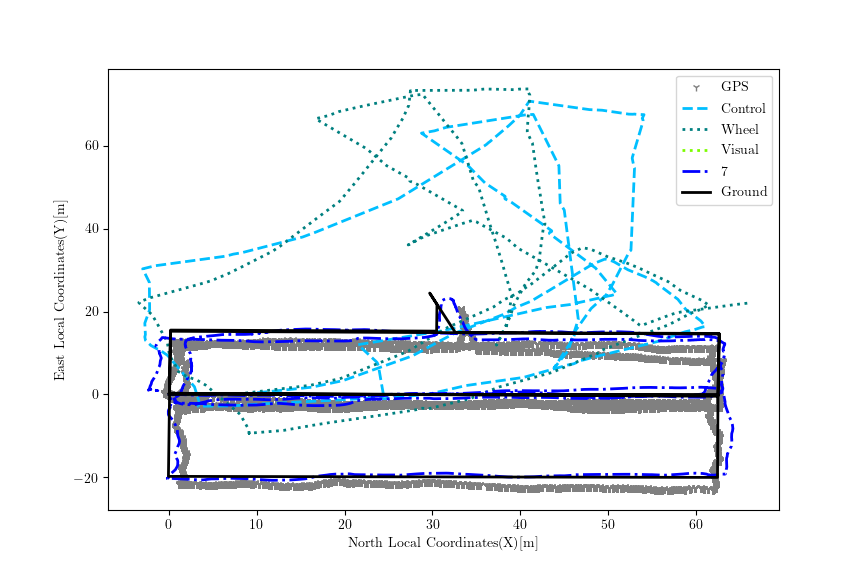
\includegraphics[clip, width=0.78 \textwidth]{Images/5-Results/GravelKF.png} %, trim=2cm 1cm 2cm 0.8cm
			\end{center}
			\caption{Best filter performance on gravel.}
	\label{fig:5-gravel}
\end{figure}
\begin{figure}[!ht]
			\begin{center}
				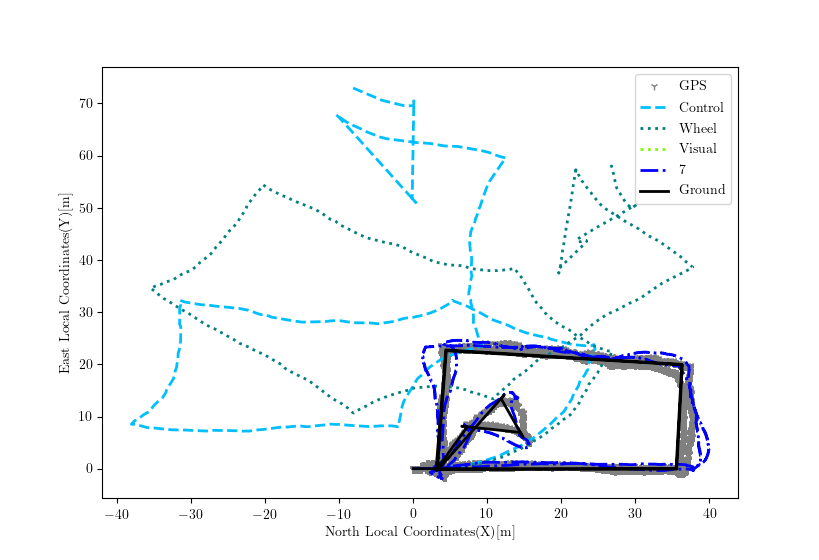
\includegraphics[clip , width=0.78 \textwidth]{Images/5-Results/GrassKF.png} %, trim=2cm 1cm 2cm 0.8cm
			\end{center}
			\caption{Best filter performance on grass.}
	\label{fig:grass-5}
\end{figure}

\com{
\begin{figure}[!ht]
	\begin{center}
		\begin{subfigure}[b]{.495\textwidth}
			\begin{center}
				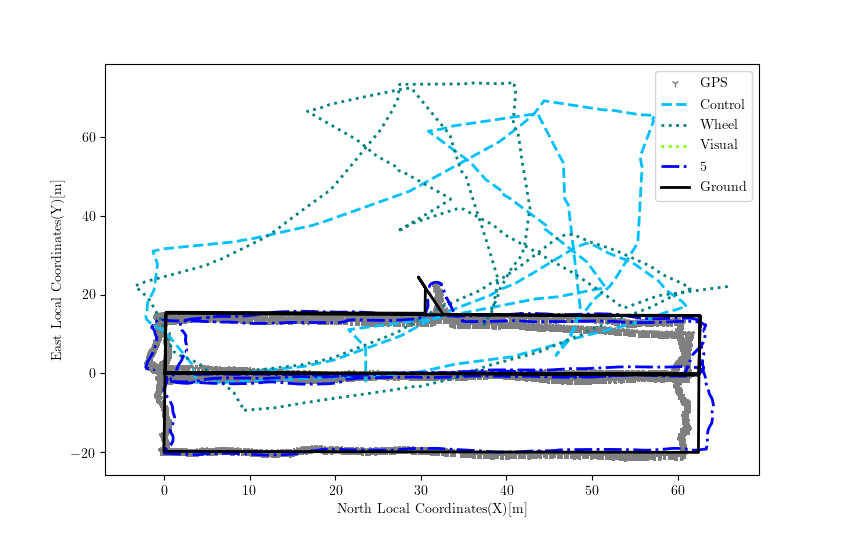
\includegraphics[clip, trim=2cm 1cm 2cm 0.8cm , width=0.8 \textwidth]{Images/5-Results/Gravel-Loc.png}
			\end{center}
			\caption{Best filter performance on gravel.}
	\label{fig:5-gravel}
		\end{subfigure}
		\begin{subfigure}[b]{.495\textwidth}
			\begin{center}
				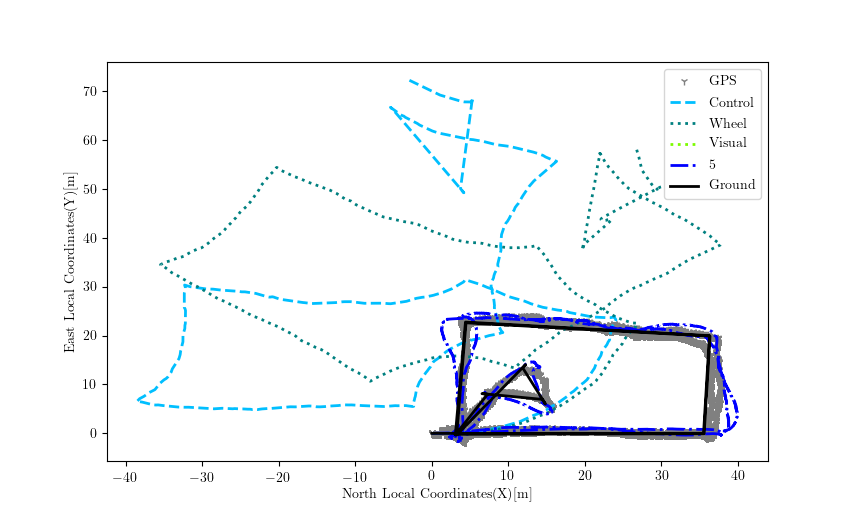
\includegraphics[clip, trim=2cm 1cm 2cm 0.8cm , width=1 \textwidth]{Images/5-Results/Grass-Loc.png}
			\end{center}
			\caption{Best filter performance on grass.}
	\label{fig:grass-5}
		\end{subfigure}%
		\caption{Localisation on grass results }
		\label{fig:camera_sensor}
	\end{center}
\end{figure}
}


\section{Mapping Analysis}
\noindent The evolution of the mapping feature is shown, from the initial setting of the occupancy grid, to the customised virtual boundary generation, and finally to the updating map behaviour.

The configuration model chosen to localise the \gls{ALM} for this module is "\textit{Model 7}", as defined in Section \ref{sec:locRes}. 
The mapping method is highly reliant on precise estimation, and the real-time requirement is especially important in case of collision events, to make sure that they are mapped to their related and timely position.

The experiments used to evaluate the mapping module are the same used for the localisation analysis, i.e., the gravel and grass experiments.
Those have been chosen for their length and completeness.
The initial test on the gravel simply defines the boundaries of the environment, defining two different zones, which could be handled differently.
On the grass test, after the virtual boundary generation, the map is also updated using eventual collision's events to account for objects present on the lawn.

The results from the map generated from the estimates provided by the localisation module are compared with a map computed with the same technique but using the ground truth trajectory.
With this approach, it is possible to check if the estimated map matches the real outdoor environment.

Their evaluation will be split between the Complete map, the Boundary definition, and the Collision identification.
On the Complete section, all the cells of the occupancy grids will be used to generate the results.
The Boundary evaluation will be computed using the cells set to the negative value $-1$, as specified, by either the ground truth or the estimate.
A similar approach will be adopted for the Collisions, using a threshold of value $25$ to distinguish between occupied and not-occupied cells.
For each category, all of the evaluation metrics defined in the methods will be performed wherever possible.

\subsection{Gravel Boundary Experiment}
\noindent
As defined before, the gravel experiment is performed to build the virtual boundary specifying two different areas.
The \gls{ALM} simply updates the cells related to its estimated pose with the negative value defined. 


The overlapped maps obtained by such a boundary definition, using both the ground truth and the \gls{EKF} estimates, are shown below in Figure \ref{fig:occGridBoud}. 
\begin{figure}[!ht]
	\begin{center}
		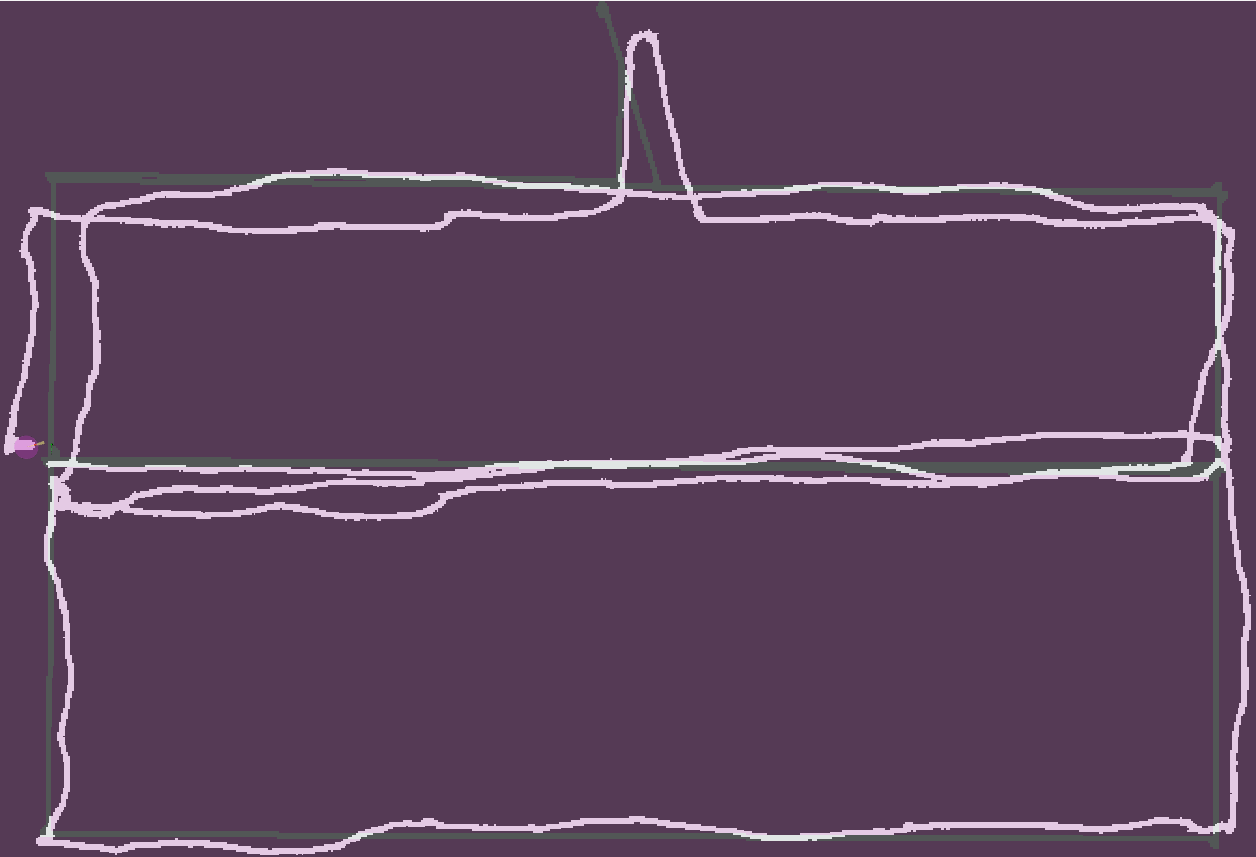
\includegraphics[width=0.7\textwidth]{Images/5-Results/Gravel5.png}
	\end{center}
	\caption{Personalised boundary definition for overlapped maps\\defined by ground truth(grey) and estimated(white).\centering}
	\label{fig:occGridBoud}
\end{figure}
%\\~\\

The results obtained by comparing the ground truth map with the estimated results are shown in Table \ref{tab:map-gravel}.\begin{table}[!ht]
	\small
	\begin{center}
		\begin{tabular}{|c||S[table-format=-1.2]|}
			\hline
			\centering{\textbf{Section}} & \multicolumn{1}{c|}{\centering{\textbf{Map Score}}}\\
			\hline
			\hline
			\centering{Complete} & 12.9    \\
			\hline
			\centering{Boundary} & 46.4  \\
			\hline
		\end{tabular}
		\caption{Gravel Mapping Results\label{tab:map-gravel}}
	\end{center}
\end{table}
\com{
\begin{table}[!ht]
	\small
	\begin{center}
		\begin{tabular}{|c||S[table-format=-1.2]|S[table-format=-0.2]|S[table-format=-0.2]|}
			\hline
			\multirow{2}{*}{\textbf{Section}} & \multicolumn{3}{c|}{\textbf{Evaluation Metric}}\\
			& \multicolumn{1}{c|}{$MS$} & \multicolumn{1}{c|}{$PCC$} & \multicolumn{1}{c|}{$F1$} \\
			\hline
			\hline
			\centering{Complete} & 12.9 & 0.27 &   \\
			\hline
			\centering{Boundary} & 46.4 & -0.69 & 0.30  \\
			\hline
		\end{tabular}
		\caption{Gravel Mapping Results\label{tab:map-gravel}}
	\end{center}
\end{table}
}

\subsection{Grass Final Experiment}
\noindent
The grass experiment evaluates the performance of the complete and final system.
It starts by building the virtual boundary running the same perimeter two times.
Afterwards, it runs inside the defined area to test the dynamic map update exploiting the collisions' sensors.
In this specific case, 3 different collision events are fired, then the \gls{ALM} is made to rotate and continue until its next collision.
At the third collision event, the mobile robot is commanded to return to its origin.


The overlapped maps obtained by such definitions using both the ground truth and the \gls{EKF} estimates are shown below in Figure \ref{fig:occGridBoud} and the related evaluation results obtained by comparing the ground truth map with the estimated results are shown in Table  \ref{tab:map-grass}.

\begin{figure}[!ht]
	\begin{center}
		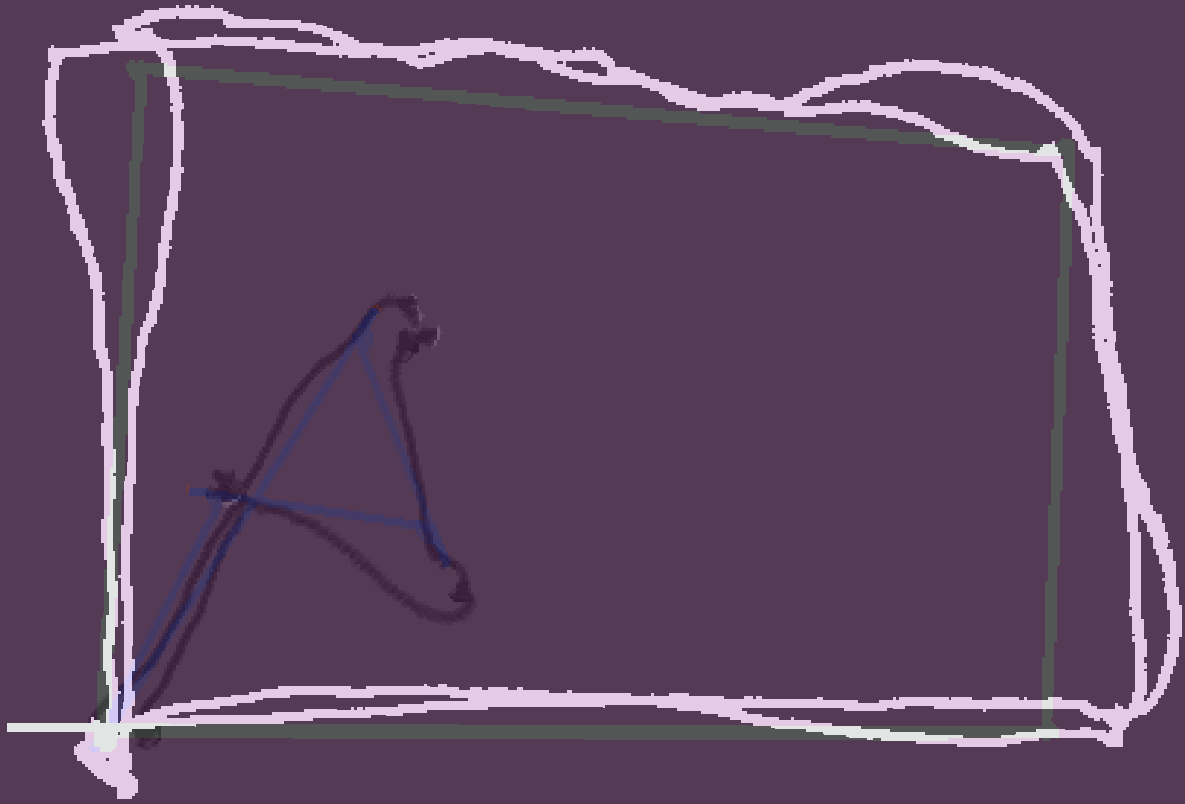
\includegraphics[width=0.75\textwidth]{Images/5-Results/Grass5.png}
	\end{center}
	\caption{Update of the map inside the boundaries (lighter shade means probability of object given by collision events)}
	\label{fig:occGridUpdate}
\end{figure}

\begin{table}[!ht]
	\small
	\begin{center}
		\begin{tabular}{|c||S[table-format=-1.2]|}
			\hline
			\centering{\textbf{Section}} & \multicolumn{1}{c|}{\centering{\textbf{Map Score}}}\\
			\hline
			\hline
			\centering{Complete} & 9.51    \\
			\hline
			\centering{Boundary} & 44.9  \\
			\hline
			\centering{Collisions} & 45.4  \\
			\hline
		\end{tabular}
		\caption{Grass Mapping Results
		\label{tab:map-grass}}
	\end{center}
\end{table}
\com{
\begin{table}[!ht]
	\small
	\begin{center}
		\begin{tabular}{|c||S[table-format=-1.2]|S[table-format=-0.2]|S[table-format=-0.2]|}
			\hline
			\multirow{2}{*}{\textbf{Section}} & \multicolumn{3}{c|}{\textbf{Evaluation Metric}}\\
			& \multicolumn{1}{c|}{$MS$} & \multicolumn{1}{c|}{$PCC$} & \multicolumn{1}{c|}{$F1$} \\
			\hline
			\hline
			\centering{Complete} & 9.51 & 0.34 &   \\
			\hline
			\centering{Boundary} & 44.9 & -0.62 & 0.35  \\
			\hline
			\centering{Collisions} & 45.4 & -0.84 & 0.07  \\
			\hline
		\end{tabular}
		\caption{Grass Mapping Results
		\label{tab:map-grass}}
	\end{center}
\end{table}
}

\subsection{Discussion on Mapping}
\noindent
The overall mapping results showcase how the generation of a reliable and accurate perception of the environment is still not possible.
This is given by the dependence on the localisation's performance, which are still not good enough to then exploit them for this purpose.

Related to the mapping module performance on its own, however, it is noticeable how effective the proposed approach could be.
The ground truth map, as obtained by using the ground truth trajectory to define both boundaries and collision events, exploits the same functionalities defined for the \gls{EKF} estimates and provides the features needed.


\cleardoublepage
%\clearpage
